% =====================================================================
% Companion report: the connectome-reservoir language model.
% Lower formality than the mechanism paper; every number is traced to a
% metrics/JSON file (earlier runs: flybrain_lm/models/*.metrics.json;
% revised runs: results/lm/*.json, script mechanism/lm_mech.py).
% =====================================================================
\documentclass[conference]{IEEEtran}
\usepackage{amsmath,amssymb,graphicx,booktabs,url,xcolor}
\usepackage[utf8]{inputenc}

\begin{document}

\title{Teaching a Fly Connectome to Predict Text: History, Audit and
Mechanism-Guided Revision of a Connectome-Reservoir Character Language Model}

\author{\IEEEauthorblockN{Quanxi Li}
\IEEEauthorblockA{Independent Researcher\\
mikey080602@gmail.com}}

\maketitle

\begin{abstract}
We drove a leaky integrate-and-fire model of the complete adult male
\textit{Drosophila} CNS connectome (MaleCNS v1.0, 166{,}700 neurons) with
character codes from TinyShakespeare and trained linear softmax readouts to
predict the next character. This report records how the project developed,
audits its earlier results, and revises the model using mechanisms identified
in a companion study. The earlier best frozen model reached 42.55\% accuracy
and 3.298 bits per character (BPC) on a 20k/5k split; adding dopamine-gated
KC$\rightarrow$MBON plasticity wrote decodable information into the synapses
but did not improve prediction, which motivated the mechanism study. The audit
finds that all plasticity results were produced on a simulator version that
wrote to the wrong synapses, and that a hashed three-character context head
alone, with no brain, reaches 42.9\% / 3.205 BPC on our 20k/5k split: the
earlier benchmark was essentially an n-gram score. The mechanism study showed
that the input used so far activates most Kenyon cells (KCs) for every symbol.
With sparse projection-neuron (PN) codes instead, the brain adds information
beyond the n-gram: on 20k/5k, KC codes plus the context head reach 43.2\% /
3.146 BPC, and all brain features 42.4\% / 3.110 BPC, the first results in the
project that improve on a context-only model. Plasticity with a uniform
teaching signal made prediction worse.
\end{abstract}

% =====================================================================
\section{Motivation}
The project began as an engineering question: can a real, frozen connectome
serve as the dynamical substrate (``reservoir'') of a language model, with only
a linear readout trained? A fly has no language circuitry; the aim was never a
claim about fly cognition but a test of how much sequence information the
wiring can carry and expose, and later of what local plasticity adds.

This language-model project came first. Its central failure, that
information written into the mushroom body by plasticity could be decoded
from the synapses but did not improve prediction, gave rise to a separate
mechanism study \cite{mechpaper}, which decomposes where such a memory is
stored, what retrieves it and how it reaches downstream neurons. This report
closes the loop: it documents the language-model history that led to that
study and then uses the mechanisms it found to revise the language model.

% =====================================================================
\section{Related work}
Using the fly connectome as a reservoir is not new. Costi et al.\ built echo
state networks from the most connected neurons of the adult fly connectome
and found them more resistant to overfitting in time-series prediction than
standard reservoirs \cite{costi2025}. The open project \texttt{fly-as-a-lm}
trains a 16{,}384-neuron subgraph of the same MaleCNS v1.0 connectome for
character- and token-level text prediction, learning the edge weights by
backpropagation while keeping the topology; its character pilot reports
45.21\% accuracy and 2.806 BPC on its own alphabet and split
\cite{flyasalm}. Our model differs in keeping the whole 166{,}700-neuron
connectome frozen, training only a linear readout, and in using local
dopamine-gated plasticity rather than gradient learning; the numbers are not
comparable. The PN$\rightarrow$KC expansion has been described as a
locality-sensitive hash that maps similar inputs to overlapping sparse KC
codes \cite{dasgupta2017}, and sparse KC codes reduce interference between
learned associations in an abstract fly model \cite{shen2023}; both anticipate
why sparse input helps below.

% =====================================================================
\section{Setup}
\textbf{Brain.} MaleCNS v1.0 \cite{berg2026} simulated with the
\texttt{flybrain} leaky integrate-and-fire package (20~ms steps, 100~ms
membrane time constant), in the spirit of whole-brain executable models
\cite{shiu2024}. \textbf{Input.} Each of the 65 characters is a fixed random
set of input channels injected for $K$ steps per character. \textbf{Readout.}
Spike traces or voltages of selected neurons, standardised, feeding a ridge or
softmax classifier for the next character. \textbf{Corpus.} TinyShakespeare
(1{,}115{,}394 characters, 65 symbols). \textbf{Metrics.} Validation accuracy
and BPC, with unigram and bigram baselines.

% =====================================================================
\section{History}
\begin{figure*}[t]\centering
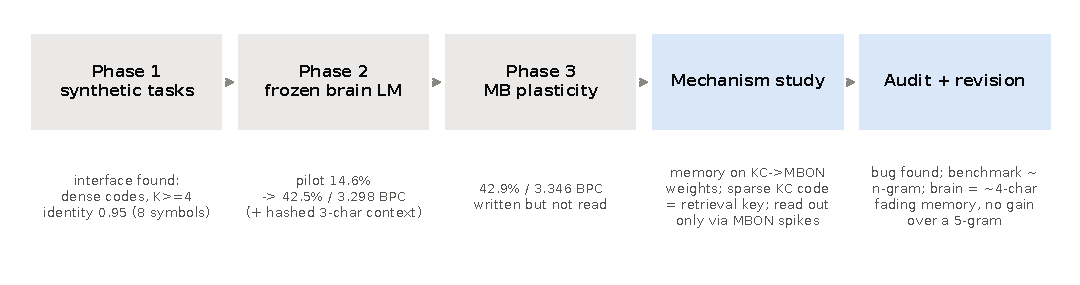
\includegraphics[width=\textwidth]{figures/fig1_timeline.pdf}
\caption{Project timeline. Gray: the language-model project (Phases 1--3);
blue: the mechanism study it led to \cite{mechpaper} and the audit and
revision reported here. Numbers are read from the metrics files.}
\label{fig:timeline}
\end{figure*}

Fig.~\ref{fig:timeline} summarises the stages.

\subsection{Phase 1: finding a usable interface (synthetic tasks)}
Early experiments on fixed-rule letter tasks failed to generalise (validation
at chance, training 0.81--0.92). Single-cell injection moved about 6 of 1{,}314
descending neurons; groups of 165 input cells moved about 30. Denser codes and
sustained injection made the symbol identity decodable across unseen noise
seeds (8 symbols: 0.48 with 32 active channels, 0.95 with 512), a
deterministic cycle task generalised (0.89, chance 0.33), and a recall task
showed a clean memory window of about two tokens.

\subsection{Phase 2: TinyShakespeare with a frozen brain}
A first pilot with two steps per character reached only unigram level
(14.6\%). Grids over steps per character, code density, input windows,
position codes, readout populations (descending, VNC, central neurons ranked
by a delayed-memory probe), voltage versus trace features, softmax readouts
and an explicit hashed order-3 character context produced the frozen
reference: 512 memory-ranked central neurons plus a 32{,}768-bucket context
head, 42.55\% / 3.298 BPC on a 20k/5k split (the project summary quotes
42.71\% / 3.227; the model's metrics file records the former).

\subsection{Phase 3: adding mushroom-body plasticity}
The author proposed using the connectome's own KC$\rightarrow$MBON synapses as
a slow memory and optimised this path over several rounds: a plastic lane on
the 61{,}210 KC$\rightarrow$MBON edges gated by simulated dopaminergic
activity, first read directly and then through small lag decoders fused with
the frozen central lane. The synaptic state was decodable, but prediction did
not improve: the best fused model reached 42.88\% / 3.346 BPC, against
42.55--42.71\% / 3.227--3.298 for the frozen reference, and direct plastic
readouts were worse (22.4\% / 9.00 BPC). This ``written but not read'' gap is
what the companion mechanism study \cite{mechpaper} set out to explain.

\subsection{Roles}
By the author's account: the research direction; the probe algorithm and its
initial parameter counts; the move from dense whole-network injection and
readout, which was slow and noisy, to sparse probe sets, which reduced the
noise; the memory-ranked readout; the experimental parameters and scale of
Phases 1--2; and the proposal to route memory through the KC--MBON synapses
were the author's. OpenAI Codex wrote the hashed context head, rewrote training
scripts for different parameter and probe-count settings and managed parallel
training runs. (The ``sparse probes'' of Phase 1 refer to how many channels
were driven and read; at the Kenyon-cell level the resulting 512-channel codes
were still dense, as the audit shows.) From Phase 3 on, the work moved beyond
what the author could direct alone: the unexplained ``written but not read''
result was pursued with a large set of AI agents, which also introduced errors
that the audit below corrects. The project log records the author's
instructions but not who proposed each idea; this division is an author
statement.% TODO(author): cite dated chats/notes for the probe design once located.

% =====================================================================
\section{Audit of the earlier results}
\begin{itemize}
\item \textbf{Wrong-synapse writes.} Every plasticity language result (all
\texttt{plastic\_*}, \texttt{pilot*} and \texttt{overnight\_*} runs) predates
the 2026-09-17 simulator fix after which plastic writes land on the intended
synapses \cite{mechpaper}. Frozen results are unaffected.
\item \textbf{The context head carries the score.} A hashed order-3 context
table initialised from smoothed counts, with no brain features, reaches
42.9\% / 3.205 BPC on our 20k/5k split. The earlier frozen reference
(42.55\% / 3.298) is therefore at the level of a pure n-gram model. Our split
differs from the earlier multi-stream sampling, so this comparison is
approximate. Consistently, the earlier same-brain model fell from 43.1\% to
22.9\% when the context head was removed (a plasticity run, hence also
produced before the simulator fix).
\item \textbf{Dense input.} All earlier runs used 512 input channels per
symbol. The mechanism study found that such codes activate most KCs for every
symbol (87\% at the probe; overlap between symbols 0.93), which removes the
sparse code the mushroom body relies on.
\end{itemize}

% =====================================================================
\section{Mechanism-guided revision}
Three changes follow from the mechanism study: (1) sparse PN codes (160 or 192
of 675 PNs, drive 1.5), where KC codes are sparse and symbol-specific;
(2) readouts that include the sparse KC code and the subthreshold MBON voltage,
since downstream spikes carry stored state only when a threshold flips;
(3) plasticity only with a teaching signal, since without dopaminergic
activity nothing is written. Each character is injected alone (no input
window), so any history must come from network dynamics. The readout is a
softmax whose hashed context table is initialised from smoothed counts on the
training rows; temperature is set on the last 10\% of the training rows; one
continuous stream; train = the first $N$ characters, validation = the next $M$.

\begin{table}[t]
\caption{Revised model. Brain features: KC counts (4{,}064), MBON voltage and
spikes (97 each), 256 MBON-target central neurons (trace and voltage).}
\label{tab:res}\centering\footnotesize\setlength{\tabcolsep}{3pt}
\begin{tabular}{@{}lcc@{}}\toprule
Model & Accuracy & BPC\\\midrule
\multicolumn{3}{@{}l}{\emph{20k/5k (bigram 27.5\% / 3.624; unigram 4.736 BPC)}}\\
Earlier frozen reference (dense input) & 42.55\% & 3.298\\
Context head only (no brain) & 42.9\% & 3.205\\
Sparse 160: KC code + context & \textbf{43.2\%} & 3.146\\
Sparse 160: all features + context, L2 $5\cdot10^{-3}$ & 42.4\% & \textbf{3.110}\\
Sparse 160: all features, no context & 38.8\% & 3.229\\
Sparse 192: all features + context & 42.2\% & 3.217\\
Sparse 192 + plasticity, teacher every token & 40.2\% & 3.450\\
\midrule
\multicolumn{3}{@{}l}{\emph{6k/2k (bigram 29.3\% / 3.747)}}\\
Context head only & 42.8\% & 3.378\\
Dense 512: all features + context & 41.1\% & 3.374\\
Sparse 192: all features, no context & 43.0\% & 3.178\\
Sparse 192: all features + context & 43.2\% & 3.147\\\bottomrule
\end{tabular}
\end{table}

\begin{figure}[t]\centering
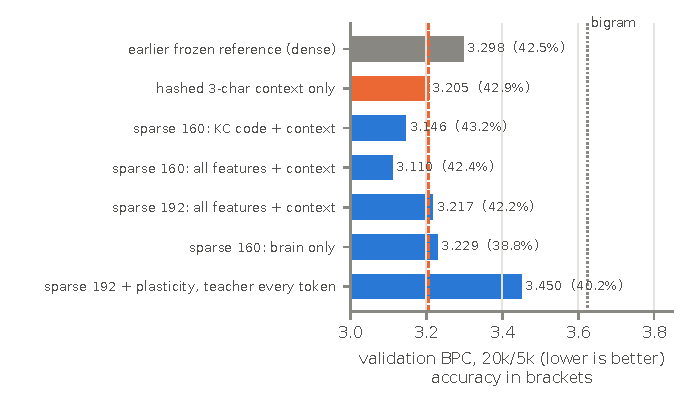
\includegraphics[width=\columnwidth]{figures/fig2_results20k.pdf}
\caption{Validation BPC on the 20k/5k split (accuracy in brackets). Dashed:
context head alone; dotted: bigram. Gray: earlier frozen reference; orange:
n-gram only; blue: revised models. Settings were chosen on the validation
split (see text).}
\label{fig:res}
\end{figure}

Table~\ref{tab:res} and Fig.~\ref{fig:res} summarise the results. On the small 6k/2k split the
sparse brain alone predicts better than the context head alone. With more
data the n-gram context becomes stronger and the brain alone falls behind it
(38.8\% / 3.229 against 42.9\% / 3.205), but combined with the context head
the sparse brain improves on it: the KC code adds 0.3 accuracy points and
0.06 BPC, all features 0.10 BPC. Dense input, which the earlier project used,
adds nothing even at 6k/2k. The KC code carries most of the brain's
contribution. Plasticity with a PAM pulse on every character wrote the
synapses (modulation up to 0.17) but made prediction worse, as expected from
the mechanism study, where a teaching signal that is the same for every item
writes changes that are not item-specific.

These gains over the n-gram are modest and come from single runs of one
seed and one text segment, and the feature set and L2 strength were chosen
by looking at the validation split, which flatters them. The readout fit is
itself noisy: refitting the sparse-160 all-feature model on the same brain
features with four different mini-batch orders gives 3.120--3.180 BPC
(s.d.\ 0.026), comparable to the gains above. A rerun with
selection on a separate held-out segment and several seeds and text offsets
is in progress. They are the first in this project that exceed a
context-only model, not evidence that the connectome models language.

% =====================================================================
\section{Discussion}
The language model did what reservoir models usually do: the explicit context
head did most of the work, and the reservoir added little until its input
regime was changed. The mechanism study explained why: dense input erases the
Kenyon-cell code that makes the mushroom body informative, and information
written into KC$\rightarrow$MBON synapses reaches downstream neurons only when
it flips an MBON spike. Using these facts turned the brain from a redundant
feature set into one that adds information to an n-gram context. The model
still does not understand language; it predicts local character structure.

\paragraph*{Limitations} One connectome; one corpus segment; short splits;
single seeds; readout settings tuned on the validation split for the 20k/5k
table (L2 and feature set), which makes the best numbers optimistic; the
revised protocol differs from the earlier one in input pathway, gain and
sampling, so comparisons with the earlier numbers are approximate.

\section*{Use of AI tools}
This is independent research by a high-school student. The author directed
Phases 1--2 and proposed the plasticity route (see Roles); from Phase 3 on,
much of the investigation was carried out by AI agents under the author's
instructions. AI agents (OpenAI Codex, DeepSeek via OpenCode, Anthropic Claude)
implemented and ran training scripts, parameter sweeps, parallel runs, audits,
and this report's analysis and drafting.

\section*{Data and code}
\url{https://github.com/LxCenady/Fly-Is-All-You-Need}.

\begin{thebibliography}{9}
\bibitem{berg2026} S. Berg \textit{et al.}, ``Sexual dimorphism in the
complete \textit{Drosophila} male central nervous system connectome,''
\textit{Cell}, vol.~189, no.~18, pp.~5504--5526.e15, 2026.
\bibitem{shiu2024} P. K. Shiu \textit{et al.}, ``A \textit{Drosophila}
computational brain model reveals sensorimotor processing,'' \textit{Nature},
vol.~634, pp.~210--219, 2024.
\bibitem{costi2025} D. Costi, A. Hadjiivanov, D. Dold, J. Hale, and D. Izzo,
``The \textit{Drosophila} connectome as a computational reservoir for
time-series prediction,'' \textit{Biomimetics}, vol.~10, no.~5, 341, 2025.
\bibitem{flyasalm} leetae9yu, ``fly-as-a-lm,'' GitHub repository,
\url{https://github.com/leetae9yu/fly-as-a-lm}, accessed 2026-09-28.
\bibitem{dasgupta2017} S. Dasgupta, C. F. Stevens, and S. Navlakha, ``A neural
algorithm for a fundamental computing problem,'' \textit{Science}, vol.~358,
no.~6364, pp.~793--796, 2017.
\bibitem{shen2023} Y. Shen, S. Dasgupta, and S. Navlakha, ``Reducing
catastrophic forgetting with associative learning: a lesson from fruit
flies,'' \textit{Neural Comput.}, vol.~35, no.~11, pp.~1797--1819, 2023.
\bibitem{mechpaper} Q. Li, ``Three addresses of a connectome-constrained
mushroom-body memory: dopamine chooses the compartment, sparse Kenyon-cell
codes set the cue, side- and subtype-specific routing shapes the output,''
2026. Mechanism study that grew out of the present project.
\end{thebibliography}
\end{document}
